----------------------------------------------------------------------
% -*-latex-*-
% Document name: controls.tex
% Creator: Rob MacLeod [macleod@vissgi.cvrti.utah.edu]
% Last update: September 2, 2000 by Rob MacLeod
%    - created
% Last update: Sun Sep 24 22:21:49 2000 by Rob MacLeod
%    -  Version 5.0Beta release edition
%%%%%%%%%%%%%%%%%%%%%%%%%%%%%%%%%%%%%%%%%%%%%%%%%%%%%%%%%%%%%%%%%%%%%%

\section{Control of \map{}}
\label{sec:control}

This section describes all the means of controlling the function of \map{},
at least all the ones we are willing to tell you about.


%%%%%%%%%%%%%%%%%%%%%%%%%%%%%%%%%%%%%%%%%%%%%%%%%%%%%%%%%%%%%%%%%%%%%%

\subsection{Control by surface}

There is an ever growing number of parameters that the user can alter
for displaying the surfaces in \map{}.  Some of the more important (and
stable) include the following:

\begin{description}
  \item [Visibility:] of points, mesh, potentials, vectors, \etc{} can all
        be controlled individually by using the appropriate function key
        (see Section~\ref{sec:control-keys}), 
  \item [Lead markings: ] of the nodes in the geometry according to their
        node number, channel number, lead number or even value,
  \item [Scaling: ] scaling of value to colour and to contour line values,
  \item [Landmarks: ] appearance of the landmarks on the surface.
\end{description}

Since this level of control is provided for each surface, it is possible to
have points showing on one surface, mesh on another, and rendered potential
shading on a third, and so on. 

\subsubsection{Selecting which surface to control} 

To control the display of each surface, be that a surface in its own window
or sharing a single window with other surfaces, a user must select that
surface.  Otherwise, display options will affect all the surfaces.  There
are two different multi-surface situations and each has its own method of
selecting the surface:
%
\begin{center}
  \begin{tabular}{|l|p{3in}|}\hline
    \multicolumn{2}{|c|}{Selecting surfaces for display controls} \\ \hline
    \multicolumn{1}{|c|}{Multi-surface layout} & 
    \multicolumn{1}{c|}{Selection method} \\ \hline
    One surface per window & Mouse location establishes currently active
    window. \\
    All surface in one window & Up/down arrows selects the surface.  Hitting
    the up-arrow key after selecting the last surface selects all surface. \\
    \hline 
  \end{tabular}
\end{center}

Note that in the surface window, the lock icons in the lower left corner
indicates if parameter settings act on all surface (locks visible) or just
single surfaces (locks invisible). Each lock controls a different aspect of 
map3d:

\begin{description}
  \item [General Lock:] is represented by the yellow (or first) lock icon.  
	When this lock is active, menu items and keyboard commands pertain 
	to all surfaces.
  \item [Transformation Lock: ] is represented by the red (or second) 
	lock icon.  When this lock is active, rotation and translation 
	pertain to all surfaces.
  \item [Frame Lock: ] is represented by the blue (or third) lock icon.
	When this lock is active, frame advancing, retreating, and resetting
	pertain to all surfaces.
\end{description}

Note: in the case where all surfaces are in the same window, when the general
lock is disabled, the active surface is displayed.  However, when the general 
lock is active and either of the other locks is disabled, the active surface
appears in a different color (blue by default), for purposes of being able to
modify one surface in comparison to the other surfaces. In this case, the +/-
keys select the surface.  + selects the next surface whereas - selects the 
previous.



%%%%%%%%%%%%%%%%%%%%%%%%%%%%%%%%%%%%%%%%%%%%%%%%%%%%%%%%%%%%%%%%%%%%%%

\subsection{Mouse control, keyboard mapping, dials, and menus}
 
Direct interactive control of \map{} is by the keyboard, mouse, and dials.
Many option are available via the menus controlled with the right mouse
button, while others can be activated or toggled with single keystrokes.
Variable (non-binary) adjustments usually occur with the dials, if they are
present, through dialogues, or by repeating keystrokes.  Below are tables
of all the current control devices and their function.  When the program
launches, the user sets one or more windows which can be resized and moved
at any time.  When launching the program with the {\tt -b} option, the
resulting borderless sub-window(s) can still be moved within a main window
using the Alt-key together with the left and middle mouse buttons.


\subsubsection{Mouse control}


The mouse can be used for different purposes depending on the current mode.
This is especially important when picking is selected.  To shift between
modes requires simultaneous pressing of the various modifier keys, shift,
control, alt. Figure~\ref{fig:mouse} shows the various actions of the mouse
buttons. 

\begin{figure}[htb]
  \centerline{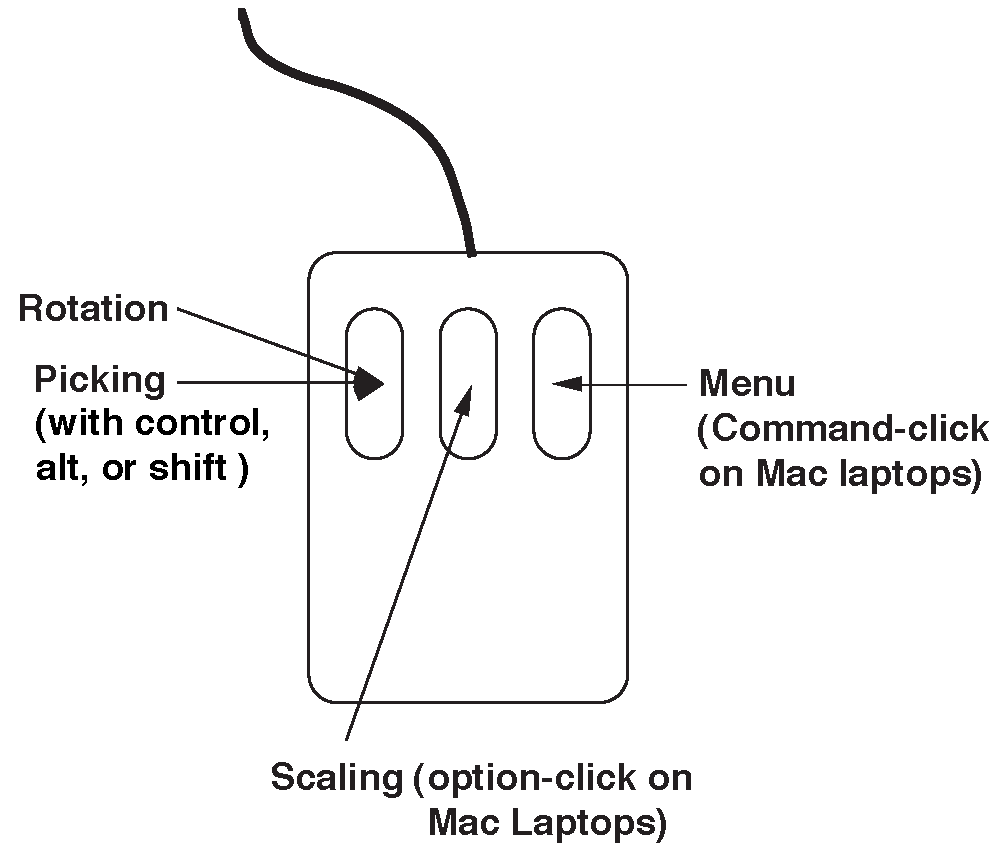
\epsfig{file=figures/mouse.epsf,height=2in}}
  \caption{\label{fig:mouse} Mouse action for \map{}.  Mouse action of both
  the left and middle mouse buttons depends on the current mode.  Picking
  makes intensive use of the mouse, as does moving objects in the surface
  window.}
  
\end{figure}

\paragraph{In surface windows: } when the mouse is over a 
surface window with a border or a surface within a borderless main window,
mouse buttons have the following actions: 
\begin{center}
  \begin{tabular}{|l|l|p{3in}|} \hline
    \multicolumn{3}{|c|}{Mouse Actions}\\
    \multicolumn{1}{|c|}{Control Key} & 
    \multicolumn{1}{|c|}{Button} & 
    \multicolumn{1}{|c|}{Action}\\ \hline
None & Left & rotation objects \\
     & Middle & scale objects (downwards increases size, upwards decreases
    size) \\ 
     & Right & activate pull-down menu \\ \hline
Cntrl & Left & pick a node (and if time series data is present, select the
    channel to display in the time series window) \\
      & Middle &  no action \\
      & Right &  no action \\ \hline
Shift & Left & translate objects \\
      & Middle & scale objects (rotates clipping planes - more info later) \\
      & Right & no action \\ \hline
\end{tabular}
\end{center}

\paragraph{In borderless windows: } when the mouse is over a 
surface within a borderless main window (-b option), the buttons have the
following additional actions: 
\begin{center}
  \begin{tabular}{|l|l|p{3in}|} \hline
    \multicolumn{3}{|c|}{Mouse Actions}\\
    \multicolumn{1}{|c|}{Control Key} & 
    \multicolumn{1}{|c|}{Button} & 
    \multicolumn{1}{|c|}{Action}\\ \hline
Alt   & Left & Move a single surface subwindow
    (no indication of motion; release to see effect) \\ 
      & Middle & Resize single surface
    subwindow (no indication of change until release of mouse button).\\
      & Right & no action \\ \hline
  \end{tabular}
\end{center}

%\newpage

\subsubsection{Keyboard controls}
\label{sec:control-keys} 

Each key of the regular keyboard, the function keys, and the keypad may be
mapped to some function of the \map{}.  Some keyboard keys serve as toggles
to change between a mode being on or off, \eg{} ``n'' toggles the display
of node markings.  Others cycle through a set of choices, \eg{} ``m'' runs
through a series of display options for the mesh.  A list of the keyboard
keys and their functions is shown in table~\ref{table:keys} and 
table~\ref{table:arrowkeys} describes the action for each of the
function and arrow keys.

% , and table~\ref{table:keypad} the actions of the keypad keys.

\begin{table}[htbp]
%\nopagebreak[4]
\begin{center}
\begin{tabular}{|l|p{4in}|} \hline
        \multicolumn{2}{|c|}{Regular keyboard} \\ \hline
        a/A-key   &       Switch colour tables \\ \hline
%        B-key	&       Toggle clipping plane \\ \hline
        c-key   &       Toggle contour draw \\ \hline
        d-key   &       Toggle depth cueing\\ \hline
%        E-key   &       Toggle backfacing visibility\\ \hline
	f-key   &	Toggle frame lock \\ \hline
%        F-key   &       Shift focus to next window \\ \hline
%	G-key	& 	Toggle display of gradients (currents) \\ \hline
%	H-key	& 	Set the location of the video box \\ \hline
	i-key	& 	Toggle ``direction'' of color table\\ \hline
        l-key   &       Toggle use of lighting\\ \hline
        m/M-key   &       Step through mesh/node drawing options \\ \hline
	n-key   &       Toggle display of node labels \\ \hline
%        O-key   &       Toggle ortho/perspective views \\ \hline
%        P-key   &       Toggle point draw \\ \hline
         Q-key   &       Quit or destroy a sub-window (Escape quits the
                         whole program) \\ \hline
        r-key   &       Reset to startup conditions \\ \hline
	S-key   &       Saves a .pts and a .fac file of the current 
	geometry \\ \hline
        s-key   &      Cycle through the various surface data draw 
        options \\ \hline
	t-key   &	Toggle transformation lock \\ \hline
%        T-key   &       Whatever Rob is currently testing \\ \hline
%	U-key	&	Toggle locking of clipping planes \\ \hline
%	V-key	&	Toggle video mode \\ \hline
%        W-key   &       Write an image to a file \\ \hline
%        X-key   &       Draw axis \\ \hline
%        Z-key   &       Rotate about z-axis in steps \\ \hline
        Escape  &       Quit the program \\ \hline
        \multicolumn{2}{|c|}{Clipping Controls} \\ \hline
	<-key	& 	Toggle front clipping plane \\ \hline
        >-key   &       Toggle rear clipping plane \\ \hline
        [/]-key   &     Move front clipping plane in (initially) +z/-z
	direction respectively \\ \hline
	{/}-key   &	Move rear clipping plane in (initially) +z/-z
	direction respectively \\ \hline
	1-key	&	Lock/Unlock clipping plane rotation with object
	rotation (when unlocked, shift-Middle-click rotates clipping
	planes) \\ \hline
	2-key	&	Lock/Unlock clipping planes from each other.
	When active, clipping planes move together \\ \hline
\end{tabular}
\end{center}
\caption{Keyboard controls in map{}.  When control contains both lower 
and upper cases of a letter, one cycles through a parameter in one 
direction and the other in the reverse direction. Note that when clipping
is active, the screen information disappears.}
\label{table:keys} 
\end{table}

\begin{table}[htbp]
\begin{center}
\begin{tabular}{|l|l|} \hline
        \multicolumn{2}{|c||}{Arrow Keys} \\ \hline
        Left Arrow Key  &       Retreat by one frame (or current frame step) \\
        Right Arrow Key &       Advance by one frame (or current frame step) \\
        Up Arrow key    &       Select next surface \\
        Down Arrow Key  &       Select previous surface \\ \hline
\end{tabular}
\end{center}
\caption{Control of \map{} via the arrow keys}
\label{table:arrowkeys}
\end{table}


%  %\medskip
%  \begin{table}[htbp]
%  \begin{center}
%  \begin{tabular}{|l|l||l|l|} \hline
%          \multicolumn{4}{|c||}{Keypad Keys} \\ \hline
%          Keypad 4  &  Y-axis rotate, CW (left) & 
%          Keypad 6  &  Y-axis rotate, CCW (right)\\ \hline
%          Keypad 2  &  X-axis rotate, CCW (down) & 
%          Keypad 8  &  X-axis rotate, CW (up) \\ \hline
%          Keypad 7  &  Z-axis rotate, CCW  & 
%          Keypad 9  &  Z-axis rotate, CW  \\ \hline
%          Keypad 1  &  Zoom down  & 
%          Keypad 3  &  Zoom up  \\ \hline
%          Keypad 0  &  Shift clip plane  & 
%          Keypad .  &  Shift clip plane  \\ \hline
%    Shft-Keypad 4  &  -X-translation (left) & 
%    Shft-Keypad 6  &  +X-translation (right)\\ \hline
%    Shft-Keypad 2  &  -Y-translation (down) & 
%    Shft-Keypad 8  &  +Y-translation (up) \\ \hline
%    Shft-Keypad 7  &  -Z-translation (away)  & 
%    Shft-Keypad 9  &  +Z-translation (towards)  \\ \hline
%          Plus key  &  Increase movement &
%          Minus Key &  Decrease movement \\ \hline
%  \end{tabular}
%  \end{center}
%  \caption{Keypad controls in \map{}}
%  \label{table:keypad}
%  \end{table}


%  \subsubsection{Dial box}
%  \label{sec:control-dials} 

%  Perhaps the most intuitive control of \map{} occurs via the dial box.  This
%  device allows ``analog'' control over any GL application that makes use of
%  dial input by allowing the user infinite control over any control parameter
%  linked to the dials.  In \map{}, the primary continuous interaction with
%  the program is in placing the object in the display, choosing the viewing
%  angle and the scale factor, and adjusting the clipping planes.  Hence these
%  functions are mapped to the dials, as described in table~\ref{table:dials}
%  and figure~\ref{fig:dials} below.

%  Note that all rotations via the dial box are relative to the screen
%  coordinate system.  This system has the x-y plane aligned with the screen,
%  the x-axis pointing from left to right, the y-axis from bottom to top, and
%  the z-axis pointing away from the viewer, perpendicular to the screen.  One
%  can picture the rotation dials as being attached to the positive ends of
%  the three axis.  See figure~\ref{fig:dials} for a description of this.

%  \begin{table}[htbp]
%  %\vspace{0.5cm}
%  \begin{center}
%  \begin{tabular}{|l|l||l|l|} \hline
%          \multicolumn{2}{|c||}{Dial Box} & 
%          \multicolumn{2}{|c|}{Mouse Control} \\ \hline
%   Dial 0 (Bottom left)    & Scale display &
%  	Left Button 	& 	Rotation/picking\\ \hline
%   Dial 1 (Bottom right)   & Clipping/z-buffer &
%  	Middle Button     &       Image scaling\\ \hline
%   Dial 2 (2nd row left)   & Z-rotate &
%  	Right Button      &       Menu selection \\ \hline
%   Dial 3 (2nd row right)  & Z-translate \\ \cline{1-2}
%   Dial 4 (3rd row left)   & Y-rotate \\ \cline{1-2}
%   Dial 5 (3rd row right)  & Y-translate \\ \cline{1-2}
%   Dial 6 (top left)       & X-rotate \\ \cline{1-2}
%   Dial 7 (top right)      & X-translate \\ \cline{1-2}
%  \end{tabular}
%  \end{center}
%  \caption{Dial controls for \map{}}
%  \label{table:dials} 
%  \end{table}

%  \begin{figure}[htb]
%  %\begin{Figure}{htb}
%  %  \NormalPicture{\columnwidth}
%  %        {3.2in}
%  %        {figures/dials.epsf}
%    \centerline{\psfig{figure=figures/dials.epsf,width=4in}}
%    \caption{Dial layout for \map{}.  Rotation dials act as if they were
%    attached to the ends of the main x, y, and z-axes, as indicated in the
%    right hand panel of the figure.}
%    \label{fig:dials}
%  %\end{Figure}
%  \end{figure}

%  %\vspace{0.5cm}

%  When more than one surface window are used, certain manipulations apply to
%  the window which currently has focus (the one in which the mouse cursor
%  sits), while others may apply to all windows synchronously.  Rotation and
%  translation can apply to one or all windows (select which via the menu or
%  F11 key), while scaling modes, colour maps, and frame numbers are applied
%  to all windows concomitantly.

\subsubsection{Menu layout}
\label{sec:control-menus}

Access to the menus is by means of the right mouse button, as per the usual
OpenGL convention.  Below is a series of tables of the menu layout for \map{}.

\begin{table}[ht]
  \begin{center}
    \begin{tabular}{|l|p{4in}|} \hline
      \multicolumn{2}{|c|}{Overview of \map{} Menus} \\ \hline \hline
      Mesh & display features of the mesh \\
      Surface Data & display features of the scalar data displayed on the
      mesh \\  
      Scaling & links between data values and color\\
      Contours & number or spacing and display features of the contours \\
      Node marking & marking of the nodes \\
      Picking & selecting times signals, mesh information, or other direct
      interactions with the display via the mouse\\
      Graphics & general display features such as lighting, clipping,
	and depth cueing \\
      Frame Controls & modifying frame controls
      Window Attributes & features of the windows such as color and text
      labels \\ \hline
    \end{tabular}
  \end{center}
\caption{The overall menu structure of \map{}}.
\end{table}


\begin{table}[ht]
  \begin{center}
    \begin{tabular}{|l|l|p{3 in}|} \hline
      \multicolumn{3}{|c|}{Mesh render menu} \\ \hline \hline
    Render as & & \\
      &  Elements  & render filled surfaces for all elements \\
      &  Connectivities & render connectivity mesh\\ 
      &  Points & render points\\ 
      &  Elements and connectivity & rendered front facing triangles as
            elements and back facing as connectivity \\ \hline 
    Line/point size 
      & \multicolumn{2}{|l|}{set the size of the points from a separate
      window}\\ \hline
    Color 
      & \multicolumn{2}{|l|}{set the color of the mesh}\\ \hline
    Secondary Mesh Color
      & \multicolumn{2}{|l|}{set color of active mesh when multiple 
	surfaces are in same window} \\ \hline
    Toggle mesh display 
      &  \multicolumn{2}{|l|}{toggle display of the mesh (without changing
          other settings)}\\ 
    \hline
    \end{tabular}
  \end{center}
\caption{Submenus for the Mesh Display menu}
\end{table}

\begin{table}[ht]
  \begin{center}
    \begin{tabular}{|l|l|p{2.5 in}|} \hline
      \multicolumn{3}{|c|}{Surface Display Menus} \\ \hline \hline
    Color & & \\
    &  Rainbow  & use rainbow color map to render scalar values on the mesh\\
    &  Green to red & use green to red color map\\
    &  Black and white & use black and white color map\\ 
    &  Invert & invert the sense of any color map, \eg{} black becomes
        white and white becomes black \\ \hline
    Render style & & \\
    &  Flat & colour each mesh element in a constant
       color according to the mean value of scalar data over the vertices\\
    &  Gouraud & shade each polygon using linear interpolation \\
    &  Banded & draw the regions between contour lines as bands of constant
       color\\  \hline
    Toggle surface display
    & \multicolumn{2}{|l|}{toggle display of the scalar data on the mesh
    (without changing other settings)}\\ \hline
    \end{tabular}
  \end{center}
\caption{Submenus to control the display of scalar data on the mesh.}
\end{table}

\begin{table}[ht]
  \begin{center}
    \begin{tabular}{|l|l|p{3 in}|} \hline
      \multicolumn{3}{|c|}{Scaling Menus} \\ \hline
    Range & & \\
    &  Local  & scale based on the local extrema for each surface and time
       instant \\
    &  Global over time series  & scale based on the extrema over the full
        times series \\ \hline
%    &  Global over surfaces & scale based on the extrema over each surface
%        for the local time instant\\
%    &  Global over everything & scale based on the extrema over all surfaces
%       and all time instants\\ \hline
    Function & & \\
    &  Linear & linear mapping between value and color \\ hline
%    &  Exponential & color changes as  $\exp({\rm value})$ \\ 
%    &  Logarithmic & color changes as  $\log({\rm value})$ \\ \hline
    Mapping & & \\
    &  True & use true extrema \\ 
%    &  Symmetric about zero & take largest of absolute values of extrema to
%       determine scaling \\
%    &  Separate about zero & scale positive and negative portions of the
%    scale independently \\ 
\hline
    \end{tabular}
  \end{center}
\caption{Menu for scaling, the mapping from data value to color for
rendering. }
\label{table:scaling}
\end{table}


\begin{table}[ht]
  \begin{center}
    \begin{tabular}{|l|l|p{2.5 in}|} \hline
      \multicolumn{3}{|c|}{Contour Menus} \\ \hline
    Number of Contours & & \\
    &  \emph{value} & selection of 5--50 contours \\
    &  Command line spacing & use the value of contour spacing in the
    \texttt{-cs} option of the command line\\ \hline
    Draw style & & \\
    & Dashed line for negative values & draw positive contours in solid,
    negative in broken lines\\
    & Solid lines for all contours & draw all contours in solid lines\\
    \hline
    Line size & \multicolumn{2}{|l|}{set the line size in a separate
    window} \\ \hline
    Toggle contours & \multicolumn{2}{|l|}{toggle display of contours
    without changing settings} \\ \hline
    \end{tabular}
  \end{center}
\caption{Menus for contour spacing/number.}
\label{table:contours}
\end{table}

\begin{table}[ht]
  \begin{center}
    \begin{tabular}{|l|l|p{3 in}|} \hline
      \multicolumn{3}{|c|}{Node Marking Menus} \\ \hline
    All & & Make all the nodes in this (or all) surface(s) \\
    &  Sphere & mark each node with a sphere \\
    &  Node \# & mark each node with the node number in the geometry \\
    &  Channel \# & mark each node with the associated data channel number \\
    &  Data value & mark each node with the associated data value \\
    &  Color & set the color for marking all nodes \\
    &  Size & set the size of all node markings \\
    &  Clear all marks & remove all node marking settings \\ 
    \hline
    Extrema & & Make all the nodes that are the extrema  \\
    &  Sphere & mark each extrema with a sphere \\
    &  Node \# & mark each extrema with the node number in the geometry \\
    &  Channel \# & mark each extrema with the associated data channel
    number \\ 
    &  Data value & mark each extrema with the associated data value \\
    &  Size & set the size of all extrema markings \\
%    &  Color & set the color for marking all extrema \\
    &  Clear all marks & remove all extrema marking settings \\ 
    \hline
    Time signal & & Make all the nodes that identify the location of time
    signals shown in the display  \\
    &  Sphere & mark each times signal location with a sphere \\
    &  Node \# & mark each times signal location with the node number in
    the geometry \\ 
    &  Channel \# & mark each times signal location with the associated
    data channel number \\ 
    &  Data value & mark each times signal location with the associated
    data value \\ 
    &  Color & set the color for marking all times signal locations \\
    &  Size & set the size of all time signal markings \\
   &  Clear all marks & remove all time signal marking settings \\ 
    \hline
    Toggle node marking & & toggle display of the selected markings \\ 
    \hline
    \end{tabular}
  \end{center}
\caption{Menus for marking nodes in the display.  If all surfaces are
currently displayed, any of these settings will affect all surfaces.  If we
have a single (or current) surface only, then change only that surface.}
\label{table:nodemarking}
\end{table}


\begin{table}[ht]
  \begin{center}
    \begin{tabular}{|l|l|p{3 in}|} \hline
      \multicolumn{3}{|c|}{Picking Menus} \\ \hline
    Size of picking aperture & & select the size of the region around the
    mouse 
    cursor that will register a ``hit'' when picking; larger values will
    make it easier to pick an object but also easier to hit multiple
    objects. \\
    Time signal & & alt-left mouse will select a time signal to show in a
    separate window\\
    & (refresh window mode) & update the last time signal window with each
    pick of a node \\
    & (new window mode) & create a new time signal window with each pick of a
    node \\ \hline
    \end{tabular}
  \end{center}
\caption{Pick mode menus.  At present, picking only selects a time signal
from the surface geometry and displays that time signal in a separate
window.  Much new functionality will be coming soon to picking.}
\label{table:picking} 
\end{table}


\begin{table}[ht]
  \begin{center}
    \begin{tabular}{|l|l|p{3 in}|} \hline
      \multicolumn{3}{|c|}{Graphics Menus} \\ \hline
    Light source & & select the source for the lighting model\\
    & From above & light shines from above the surface \\
    & None & no lighting (turn lighting off) \\ \hline
    Toggle clipping & & toggles particular clipping plane options
    & Front plane & toggles front clipping plane
    & Back plane & toggles rear clipping plane
    & Locking planes together & makes planes translate together
    & Locking planes with object & rotate surface with the planes or
	rotate surface through the planes \\ \hline
    Depth cue & & apply depth cueing (fog) \\
    & Turn on & switch depth cueing on \\
    & Turn off & switch depth cueing off \\
    \hline
    \end{tabular}
  \end{center}
\caption{Graphics menus.  These control general graphic rendering options.}
\end{table}

\begin{table}[ht]
  \begin{center}
    \begin{tabular}{|l|l|p{3 in}|} \hline
      \multicolumn{3}{|c|}{Frame Controls Menus} \\ \hline
    Lock Frames  & \multicolumn{2}{|l|}{toggle whether frames 
	operations affect one surface or all surfaces} \\ \hline
    Set Interval Between Frames & &
      & \emph{value} & select between 1 and 90 for frame animation step \\
      & Command Line Interval & use the value of interval specified in the 
	-i option of the command line \\ \hline
    Reset Frames to 0 & positions the surface at the first position in time
	\\ \hline
    \end{tabular}
  \end{center}
\caption{Controls for the attributes of the map3d windows.}
\end{table}


\begin{table}[ht]
  \begin{center}
    \begin{tabular}{|l|l|p{3 in}|} \hline
      \multicolumn{3}{|c|}{Window Attributes Menus} \\ \hline
    Screen info & & select the text written to the screen\\
      & Turn screen info on & \\
      & Turn screen info off & \\ \hline
    Color & & select window colors with the separate color selector \\
      & Background & select background color for the window \\
      & Foreground & select foreground color for the window \\ \hline
    Size & & select some size options \\
      & Double current size & double the current window size \\
      & Half current size & half the current window size \\ \hline
    Toggle Transformation Lock & toggle whether surfaces transform 
	together or independently \\ \hline
    Save Mesh & save the current position of the surface in a .pts and a .fac
	file \\ \hline
    \end{tabular}
  \end{center}
\caption{Controls for the attributes of the map3d windows.}
\end{table}



%  Report level & & \\
%     & \multicolumn{2}{l|}{Level 0 = default} \\
%     & \multicolumn{2}{l|}{Level 1 = report extrema} \\
%     & \multicolumn{2}{l|}{Level 2 = mild debugging}  \\
%     & \multicolumn{2}{l|}{Level 3 = moderate debugging} \\
%     & \multicolumn{2}{l|}{Level 4 = max debugging} \\ \hline
%  \hline
%Save settings & & \\
%   & \multicolumn{2}{l|}{save in local .map3drc} \\
%   & \multicolumn{2}{l|}{save in home .map3drc} \\ \hline

%%%%%%%%%%%%%%%%%%%%%%%%%%%%%%%%%%%%%%%%%%%%%%%%%%%%%%%%%%%%%%%%%%%%%%

%  \subsection{Feedback Reporting Level}

%  In order to control the amount of printed feedback \map{} provides (which
%  is posted in the window from which the program was launched), the user can
%  select a value between 0 and 3 from the a sub-menu of the main menu titled
%  {\em Report level}.  The settings and level of output are as follows:

%  \begin{center}
%  \begin{tabular}{|c|l|} \hline
%    \multicolumn{1}{|c|}{Report Level} &
%    \multicolumn{1}{|c|}{Types of output} \\ \hline
%    0 & minimal output --- just changes in status \\
%    1 & report extrema \\
%    2 & report some warning messages \\
%    3 & debug mode \\ \hline
%  \end{tabular}
%  \end{center}


%%%%%%%%%%%%%%%%%%%%%%%%%%%%%%%%%%%%%%%%%%%%%%%%%%%%%%%%%%%%%%%%%%%%%%

\subsection{Controlling the time signal window}
\label{sec:control-scalar} 


There are two ways to create a time signal window:
%
\begin{enumerate}
  \item Specify a \texttt{-at xmin xmin ymin ymax} on the command line
        (optionally with a \texttt{-t trace-lead-number} to specify the
        channel to use).
  \item Using picking to select a lead to show in the time signal window.
        Note that subsequent time signal picking can be set to either a)
        update the last time signal window to the new data channel or b)
        add yet another time signal window.
\end{enumerate}
%

The format of the scalar display is fairly simple 
%(see Section~\ref{sec:displayscalar})
, with a vertical bar moving along the time axis as the frame number is
advanced.  \map{} derives the time axis label from the frame numbers of the
signal relative to the time series data file, not relative to the subset of
frame read in, \ie{} if frames (or pot file numbers) 10--20 are read in
with an increment of 2, then frame number will begin at 10, and go through
12, 14, 16, 18 and end at 20 rather then beginning at 0 or 1 and going to 10
(the number of frames of data actually read).

There is also a menu item for adjusting the time base of the signal,
manually aligning time across multiple windows, and setting the time
increment between frames of data.

\subsubsection{Adjusting the frame marker}

In order to facilitate rapid movement through large datasets, the user can
control the frame number being displayed by interacting with the scalar
window itself.  If the user moves the cursor to the scalar window and
pushes the left mouse button, the vertical time bar will jump to the
nearest sample to the cursor location.  The user can then hold the left
button down and slide the time marker left and right and set a desired
frame.  Once the mouse button is released,\map{} updates the map display.
The left and right arrow keys also shift the frame marker back and forth.
The only other command allowed when the cursor is within the scalar window
is the ``q''-key, to shut down just the scalar window, or the ``f'' key,
to toggle the frame lock.  Any other attempt at input will not be accepted.


%%%%%%%%%%%%%%%%%%%%%%%%%%%%%%%%%%%%%%%%%%%%%%%%%%%%%%%%%%%%%%%%%%%%

\subsection{Picking mode}
\label{sec:control-picking} 

By ``picking'' we mean selecting some piece of the display in the current
window using the mouse (with buttons).  \map{} will eventually support
selection of a number of different elements of the display: nodes,
triangles, scalar leads, \etc{} all of which either return some
information, or affect the display, or even the geometry of the display.
In version 5.0Beta, the choices are limited to node information and a time
signal.  To control picking, use the top-level ``Picking'' menu. See
Table~\ref{table:picking} for the available options.


% and then one of the choices in the
% ``Toggle Pick Action'' submenu. Below we describe each of the picking
% option in more detail.

%  To adjust the size of the picking window, the keypad plus/minus keys can be
%  used, much as they are to alter the sensitivity of the dials to rotation
%  and translation.  Experience suggests that a larger window makes
%  triangulating (selecting nodes) easier while a small window makes selecting
%  triangles (to remove or flip them).  Each picking mode maintains its own
%  picking window size so that changes affect only the current picking mode.

\subsubsection{Picking Nodes}

This mode simple returns the location, in the same coordinates in which the
point  data was originally read into the program (the points are shifted to
keep the object at the center of the screen's coordinate system).

%  \subsubsection{Picking Triangles}

%  When simple triangle picking is selected, the node numbers of each of the
%  vertices of the triangle are displayed, along with the coordinates of the
%  nodes at those vertices.

%  \subsubsection{Triangulating}
%  \label{sec:triangulate} 

%  You can edit the triangulation of the mesh by selecting the ``Triangulate''
%  option from the ``Toggle Pick Mode'' submenu.  In this mode, the left mouse
%  is used to select the nodes that you wish connected into a triangle.  Note
%  that the cursor changes each time you select a valid point (see
%  figure~\ref{fig:triangulate}).  If there is no change,then you either hit no
%  points, or two points.  Adjust the display, or the sensitivity of the
%  picking window (keypad plus/minus keys) and try again.  The window from
%  which \map{} was launched will tell you more, and on the Indigo(s), sound
%  effects provide audio feedback.

%  \begin{figure}[htb]
%  %\begin{Figure}{htb}
%  %  \NormalPicture{\columnwidth}
%  %        {3in}
%  %        {figures/triangulate.epsf}
%    \centerline{\psfig{figure=figures/triangulate.epsf,width=\columnwidth}}
%    \caption{Triangulation modes and cursor changes.  Before picking the
%    first point of the triangle, the cursor is a short cross-hair.  After
%    successful picking of the first point, the cursor gets a horizontal mark
%    (one side of the triangle) added.  Selecting the second point adds
%    another side to the triangle and picking the third point returns to the
%    original cross-hair.  Always pick in a counterclockwise pattern as seen
%    from the outside of the surface for proper triangle orientation.  The
%    middle mouse can be used to remove a triangle from the mesh.}
%    \label{fig:triangulate}
%  %\end{Figure}
%  \end{figure}

%  Pushing the middle mouse button selects the nearest triangle and kills it,
%  removing it from the list.

%  Files with the latest version of the connectivity are updated each time you
%  leave triangulate mode, which you can do by either hitting the ``Q'' key or
%  selecting ``Turn picking off'' option.  The filenames are created in a
%  random fashion and are (optional) removed when you end the session and
%  save the latest version of the geometry in a file of you choice.  When you
%  go to exit \map{}, you will be asked for the basefilename into which you
%  wish the updated version of all surfaces (points and connectivities) to be
%  stored.  At the moment, these files are .pts/.fac files, which can easily
%  be converted to .geom files if needed.  

%  \subsubsection{Triangle flipping}

%  Often it is necessary to know the orientation of the triangles in the
%  geometry.  While this can be computed, there remains a 180-degree ambiguity
%  as to which way the normal points.  To resolve this, triangles nodes should
%  be ordered in a counterclockwise direction as viewed from the ``outside''
%  of the surface to which the triangle belongs.  This convention is used by
%  GL to decide which triangles to show in ``hide backfacing triangles'' mode
%  (which you can toggle with the E-key in \map{}).  Unfortunately, it is not
%  always possible when constructing geometric models to tell which way the
%  triangle is to be viewed --- this is still something humans do better than
%  computers --- and so we often need to edit a geometric model so that the
%  triangles are 'flipped' the right way.  Hence, the ``Flip triangle'' option
%  in the ``Toggle Pick Action'' submenu.

%  To check a model for correct triangle orientation and flip the offending
%  triangles, select ``Flip triangle'' from the ``Toggle Pick Action''
%  submenu.  The cursor will change shape (to a cross-hairs with triangle
%  around it) and \map{} will go into ``hide backfacing triangles'' mode.
%  This means that only the front-facing triangles are drawn and the holes
%  indicate which triangles need flipping.  Then the cursor in each triangle you
%  want to flip and hit the left mouse button.  If you were successful, the
%  triangle will fill in.

%  This option, like triangulating, produces a new connectivity file, which is
%  saved temporarily in a random filename each time you leave triangle-flip
%  mode.  When the program finishes, you will be prompted for the base
%  filename of a new set of points and fac files, thus preserving the original
%  files for later use.

%%%%%%%%%%%%%%%%%%%%%%%%%%%%%%%%%%%%%%%%%%%%%%%%%%%%%%%%%%%%%%%%%%%%%%%%%%
%  \subsection{Editing Geometry}

%  \map{} provides a number of tools for editing the geometry at the heart of
%  the display and also saving those changes in new versions of the geometry
%  files.  An example of this is described in the previous
%  section~\ref{sec:triangulate} for altering the node connectivity.  Other
%  examples include the ability to apply the current viewing transformation to
%  the geometry and save the result, typically for use in another graphics
%  program (see section~\ref{sec:geom-transform}). 

%  \subsubsection{Applying transformations to data}
%  \label{sec:geom-transform}

%  \paragraph{Background: }The idea of this feature is to be able to apply the
%  same translations and rotations that are possible within \map{} to the
%  geometry data itself, and save the result for use elsewhere.  The
%  application was to produce 2D projections from 3D meshes and save the
%  results in a projection that made it useful for 2D plotting programs like
%  the infamous {\em Z\/} and less famous {\em pscont}.

%  \paragraph{Usage: } Access to this command is from the menu, and requires
%  the following steps:
%  %
%  \begin{enumerate}
%    \item Bring up the geometry and select the surface(s) to be transformed.
%    \item Rotate and translate until the desired project (view) of the
%          geometry is fixed.
%    \item Select from the main menu, the ``Rotation/Translation'' submenu,
%          then the ``Apply Current Rotation to Geometry'' choice.
%    \item This will cause only subtle visible changes on the screen, but if
%          the axis are turned on (X-key), they will flip back to the default
%          position, while the image of the geometry remains fixed, a sign
%          that translations have been applied to the geometrical data and not
%          just the transformation matrices maintained within \map{}.
%    \item When leaving \map{}, make sure you check the window from which it
%          was launched for the dialog that directs the saving of the
%          transformed data in a new file.  Choices include the geometry file
%          form (.pts/.fac or .geom) (see section~\ref{sec:geomfiles} for
%          detail) and the basefilename, to which appropriate suffix(es) are
%          applied to make the final filename(s). 
%  \end{enumerate}

%%%%%%%%%%%%%%%%%%%%%%%%%%%%%%%%%%%%%%%%%%%%%%%%%%%%%%%%%%%%%%%%%%%%%%
%  \subsection{Control of landmark display}
%  \label{sec:control-landmarks} 

%  Landmark shading can be altered
%  with some cheap lighting tricks to give a variety of different
%  appearances.  These tricks are cheap in the sense that they were
%  relatively easy to implement but also in that they require minimal
%  computational overhead.  To play with the display options of the landmarks,
%  select the ``Drawing Landmarks'' menu option, then one or more of the
%  lighting models and colours.  The options are set up as follows:
%  %
%  \begin{description}
%    \item [Draw default shaded landmarks:] this is the same mode as was used
%          previously. 
%    \item [Draw eye-point shaded landmarks: ] this is the simplest of light
%          models in which the colour shading varies with angles away from a
%          line between an imaginary eye location and the center of the
%          object.  Use this,together with the ``Select eye-point location''
%          item to give a different look to the landmarks.
%    \item [Landmark shading colour: ] This selects the colour used to draw
%          the landmarks.  There are only a few basic colours implements at
%          the moment, but this can be expanded at any time.  Note that by
%          interactively altering the colour map, different colours can be
%          tested, but only with major limitations since the colour intensity
%          varies with the lighting model.
%    \item [Draw mesh landmarks: ]  This mode is primarily for debugging the
%          definition files for the landmark files and shows each landmark in
%          its elemental segments, with labeling of each segment.
%    \item [No landmarks: ] As before, this option turns off display of the
%          landmarks.
%    \item [Draw plane: ] switches the display of any landmark planes in
%          the landmark files on and off.
%    \item [Plane colour: ] selects the colour to be used to draw the landmark
%          plane. 
%  \end{description}


%%%%%%%%%%%%%%%%%%%%%%%%%%%%%%%%%%%%%%%%%%%%%%%%%%%%%%%%%%%%%%%%%%%%%%%%
